%%=============================================================================
%% Analyse marketing Kriket
%%=============================================================================

\chapter{Kriket analyse}
\label{ch:analyse}

Nadat Michiel en Anneleen, de oprichters van Kriket, succesvol een crowdfunding\footnote{Via \href{https://www.growfunding.be/nl/bxl/kriket}{growfunding.be} konden Michiel en Anneleen 13.275 euro verzamelen met steun van 254 growfunders.} afsloten op 11/07/2017 was er al een community onstaan. Deze kleine community is ontstaan door mond to mond reclame, wat de beste reclame is.

Het maken van de krekelrepen deden ze zelf in een kleine DIY (do it yourself of in het Nederlands: doe het zelf) keuken voor een heel jaar, terwijl dat de crowdfunding aan het lopen was. Zo konden ze mensen warm te maken voor dit nieuwe concept. Vanaf oktober 2018 begon Kriket met productie, ze lanceerde een webshop en gingen op zoek verschillende lokale verdelers die hun krekelrepen in de winkels wouden leggen.  

\begin{figure}[h!]
	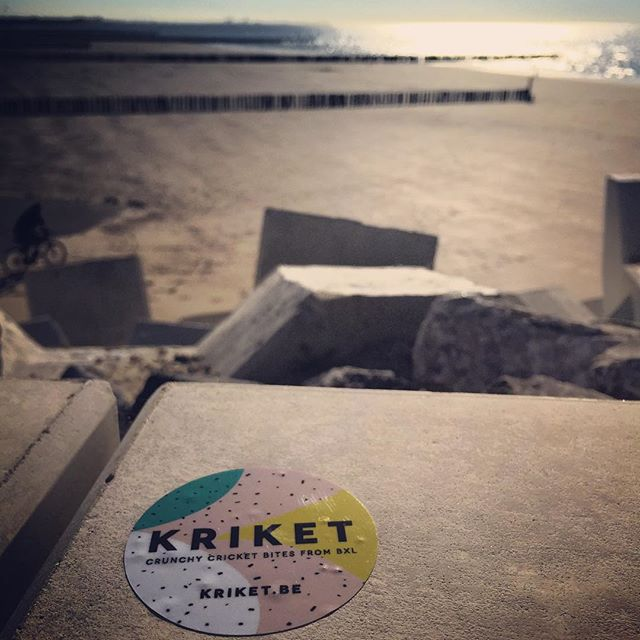
\includegraphics[width=100mm]{img/stickerguerilla.jpg}
	\centering
	\caption{Via Instagram ziet men ook dat er in het begin (27 mei 2017) aan ``stickerguerilla`` werd gedaan}
	\label{fig:stickerguerilla}
\end{figure}

\section{Huidige marketingsituatie}
\label{sec:huidige-marketingsituatie}
Om andere mensen mee te krijgen in het verhaal van Kriket (want het is niet zomaar een krekelreep) geven ze geregeld gratis proevers weg bij één van hun verdelers. Dit wordt gepost op sociale media en zo hebben ze meteen enkele fans die dit kunnen doorvertellen. Tezamen met de mensen die dan toevallig in die winkel hun eten komen kopen kunnen ze het verhaal van Kriket vertellen en eventueel enkele van de repen verkopen.

Dit zorgt dan weer voor mond tot mond reclame, want ``Ik heb vandaag in de winkel een krekelreep gegeten. Je smaakt die krekels niet, het is gewoon heel lekker en gezond!`` wordt thuis doorverteld, of aan vrienden. 

Kriket heeft een duidelijke en goede communicatie op Facebook en Instagram, het leunt nauw aan bij het product dus daardoor past het allemaal mooi samen. Instagram stories worden ook zeer correct gebruikt en geven dus informatie die tijdelijk of heel relevant is op het moment van publicatie. Alle communicatie gebeurt in het Engels, hiermee kan iedereen van hun doelgroep begrijpen wat ze willen delen, zowel de Nederlandstaligen als Franstaligen binnen België en ook alle buitenlanders. De website \href{https://kriket.be}{kriket.be} is wel drietalig, hierop kunnen de krekelrepen gekocht worden samen met enkele goodies zoals een T-shirt, pet of tote bag. 

De webshop wordt via sociale media af en toe vermeld, maar het is niet het voornaamste kanaal dat ze gebruiken om de krekelrepen te verkopen.

Naast de lokale verdelers kon Kriket bij AVEVE, Carrefour en Delhaize een plaatsje vinden. De krekelrepen kregen (gratis) publiciteit op TV en ze stonden op verschillende vernieuwende events over ``The Food of the Future``. Ook staat Michiel met verschillende interviews in kranten en tijdschriften, zoals die van UNIZO, Bloovi, enz. De krekelrepen zijn zelfs te vinden in een automaat op een middelbare school.

Er wordt ook geëxperimenteerd met influencer marketing, dit doet Kriket met twee sportieve dames, Aline en Tiphaine. Ze plaatsen enkele posts op hun Instagram account en delen een kortingscode via Instagram stories.

\begin{figure}[h!]
	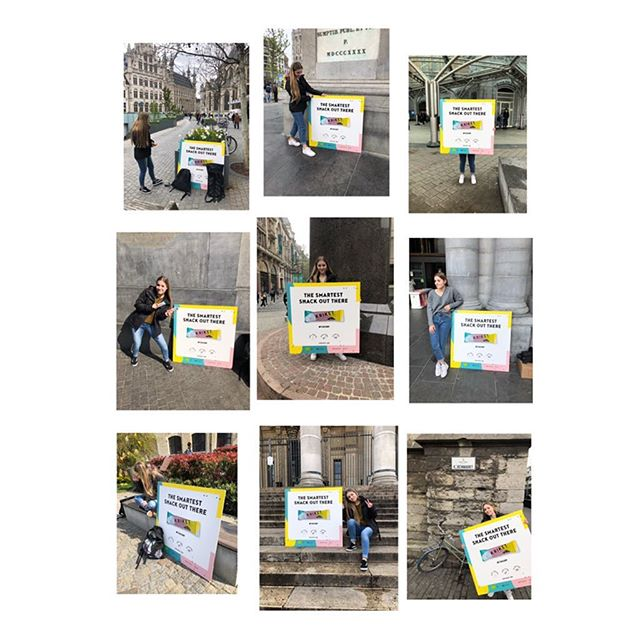
\includegraphics[width=150mm]{img/kriket-on-tour.jpg}
	\centering
	\caption{Kriket on tour, met een groot Kriket-bord en gratis krekelrepen.}
	\label{fig:kriket-on-tour}
\end{figure}

Toen Kriket 2 nieuwe producten aankondigde deden ze dit op een originele manier. Via Facebook en Instagram telden ze de laatste 3 dagen af om de volgers warm te maken voor de nieuwe krekelrepen. Op de dag dat ze waren aangekondigd ging Kriket rond Vlaanderen; Antwerpen > Gent > Brussel > Mechelen > Leuven. Hier stonden ze met een groot bord en gaven ze gratis repen als promotie voor de twee nieuwe krekelrepen. Dit kan je plaatsen zien als een goede uitvoering van guerillamarketing.

Kriket speelt ook in op de actualiteit, zoals de klimaatmarsen, want de repen van Kriket worden lokaal geproduceerd. Ze zijn ook een goed alternatief voor vlees als bron van proteïnen. Krekels zetten voeder 10 keer efficiënter om in eiwit dan koeien. Verder nog, ze consumeren 300 keer minder water en stoten 60 keer minder broeikasgassen uit \autocite{Kriket2018}.

Verder neemt Kriket ook deel aan wedstrijden, dit zorgt ook steeds voor publiciteit. Zoals de NX-food start-up wedstrijd, deze hebben ze gewonnen en hieruit hebben ze een overeenkomst met Eurowings kunnen maken \autocite{KriketEurowings2019}.

Eurowings is een heel interessante partner, want dit vakantiegevoel dat mensen hebben op het vliegtuig gaat goed samen met het ``avontuurlijke`` van Kriket. Mensen gaan vaker iets nieuw proberen in zo'n situatie. Dit koppelt een goed gevoel met Kriket, wat ideaal is.

Tijdens het schrijven van deze bachelorproef kwam Kriket met steeds meer uitvoeringen van ideeën die tijdens de literatuurstudie en interviews naar boven kwamen. De opsomming hiervan wordt in het volgende hoofdstuk besproken.